\subsection{Elektronik}

\author{Ervin Mazlagi\'c}

\begin{frame}
	\frametitle{Übersicht\hfill{}\footnotesize \group}
\end{frame}

\subsubsection{Fachgruppe ET}
\begin{frame}
	\frametitle{Fachgruppe ET\hfill{}\footnotesize \group}
	\begin{columns}
		\begin{column}{0.5\textwidth}
				\textit{``Denn es ist eines ausgezeichneten
					Mannes nicht würdig, wertvolle Stunden
					wie ein Sklave im Keller der einfachen
					Berechnungen zu verbringen''}
				~ \\ ~ \\
				\hfill{} -- Gottfired Wilhelm Leibniz
		\end{column}
		\begin{column}{0.5\textwidth}
			\begin{block}{Ziele}
				\begin{itemize}
					\item Synergien nutzen
					\item Austausch ermöglichen
					\item Eigenentwicklungen
					\item Shared-Dokumentationen
					\item OpenHardware
				\end{itemize}
			\end{block}
			\begin{exampleblock}{github.com/pren-et}
				\begin{itemize}
					\item 7 Contributors
					\item 7 Repositories
					\item 4 Dokumentationen
				\end{itemize}
			\end{exampleblock}
		\end{column}
	\end{columns}
\end{frame}

\subsubsection{Motoren}
\begin{frame}
	\frametitle{Motoren\hfill{}\footnotesize \group}
	\framesubtitle{Schrittmotor (Stepper) für Turmausrichtung}
\end{frame}

\begin{frame}
	\frametitle{Motoren\hfill{}\footnotesize \group}
	\framesubtitle{Synchronmotor (BLDC) für Ballwurf}
\end{frame}

\begin{frame}
	\frametitle{Motoren\hfill{}\footnotesize \group}
	\framesubtitle{Gleichstrommotor (DC) für Ballnachführung}
\end{frame}

\subsubsection{Mikrocontroller}
\begin{frame}
	\frametitle{Mikrocontroller\hfill{}\footnotesize \group}
	\framesubtitle{Freedomboard FRDM-KL25Z}
	\begin{columns}
		\begin{column}{0.5\textwidth}
			\begin{figure}
				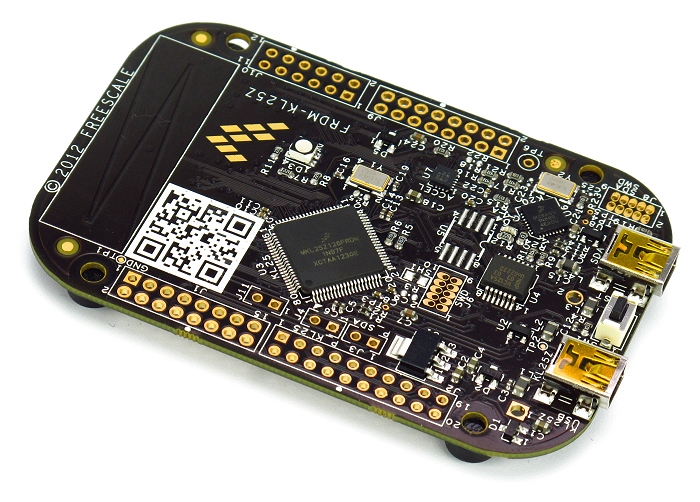
\includegraphics[width=1\textwidth]{../../fig/frdm-kl25z.jpg}
			\end{figure}
		\end{column}
		\begin{column}{0.5\textwidth}
			\begin{itemize}
				\item LowLevel-Schnittstelle für
					\begin{itemize}
						\item Motoransteuerung
						\item Sensorik \& Messtechnik
						\item Busse (UART, SPI, I$^2$C)
					\end{itemize}
				\item Programmierung in C
				\item Kommunikation über UART
				\item Programmierung mit CW, KDS oder GCC möglich
			\end{itemize}
		\end{column}
	\end{columns}
\end{frame}

\subsubsection{Messtechnik}
\begin{frame}
	\frametitle{Messtechnik\hfill{}\footnotesize \group}
	\framesubtitle{Halleffekt-Schalter als Drehgeber}
\end{frame}
